\chapter{Descripción de los algoritmos}
Para aclarar ciertas cuestiones referentes a las soluciones en este tipo de algoritmos estocásticos de tipo evolutivo, si no se especifica un tipo de representación se da por hecho que las soluciones se representan como vectores en un espacio $n$-dimensional. Un conjunto de individuos/vectores dan como resultado una población. La población es una matriz de $N\times M$, donde $N$ es el número de filas o número de individuos en la población y $M$ es el número de características del problema ($M$ dimensiones). Algunos algoritmos admiten codificación binaria y otros continua, ese tipo de cuestiones si serán especificadas.\\[6pt]
Por lo general, excepto para los algoritmos \textbf{GA} y \textbf{ACO}, se utilizarán funciones de transferencia a la hora de modificar los algoritmos para su versión binaria, tal y como se ha mencionado en el repaso bibliográfico.
\section{Algoritmos genéticos}
\subsection{Introducción}
Los algoritmos genéticos están inspirados en la selección natural y se utilizan tanto en problemas de optimización con restricciones como sin ellas. Es una metaheurística que modifica una población de soluciones individuales de manera repetida, seleccionando soluciones ``padre'' que dan lugar a la siguiente generación de soluciones en la siguiente iteración del algoritmo. En su forma más básica, un algoritmo genético opera sobre una población de soluciones potenciales a un problema dado. Cada solución potencial, a menudo llamada individuo o cromosoma, está representada como una cadena de símbolos, que puede ser binaria, numérica o simbólica~\cite{10.5555/522098}.

\subsection{Funcionamiento y Operadores}
Las soluciones o \textbf{fenotipos} están compuestas por una serie de propiedades, características, cromosomas o \textbf{genotipos}, que pueden ser mutados y alterados. La representación más común es la binaria, pero otras codificaciones son posibles.

El proceso típico incluye~\cite{mathew2012genetic}:
\begin{itemize}
    \item Inicialización aleatoria de la población.
    \item Evaluación del \textit{fitness} de cada individuo.
    \item Selección de padres basada en el \textit{fitness}.
    \item Creación de una nueva generación mediante cruces y mutaciones.
    \item Elitismo: selección de los mejores individuos~\cite{mirjalili2019genetic}.
\end{itemize}

\begin{figure}[htp]
    \begin{center}
        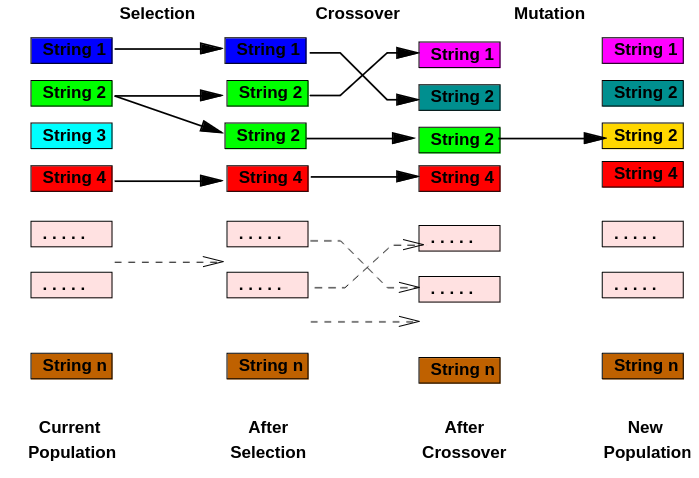
\includegraphics[width=0.6\textwidth]{imagenes/ga-working-principle.png}
    \end{center}
    \caption[Funcionamiento de un algoritmo genético]{Figura obtenida de \cite{mathew2012genetic}}
\end{figure}


El algoritmo termina cuando se alcanza cierta tolerancia de error o número máximo de iteraciones.

\subsubsection{Selección}
La selección se puede llevar a cabo con varios métodos, uno de los más utilizados en selección por torneo.\\[6pt]
En la selección por torneo, los individuos compiten entre sí en grupos pequeños. Cada grupo (torneo) tiene varios competidores (individuos). El competidor con la mejor aptitud (\textbf{fitness}) dentro del grupo tiene más probabilidad de ganar. Los ganadores son seleccionados para ``reproducirse''. Este proceso se repite hasta que se completa el \textit{pool} de apareamiento con los ganadores de los torneos~\cite{miller_genetic_nodate}. La probabilidad de cada individuo en base a su \textbf{fitness} se calcula de la siguiente manera:
\begin{equation}
    P(\text{parent}_i) = \frac{\text{fitness}(\text{parent}i)}{\sum_{j=1}^{N} \text{fitness}(\text{parent}_j)}
\end{equation}

Para las versiones binaria y continua del algoritmo se utilizan diferentes operadores de mutación y cross-over.

\subsubsection{Cruce binario}
\textbf{One-point crossover}: Se elige al azar un punto en los cromosomas de ambos progenitores y se designa como "punto de cruce". Los bits a la derecha de ese punto se intercambian entre los dos cromosomas parentales. El resultado son dos descendientes, cada uno con información genética de ambos progenitores~\cite{DAGDIA2020283}.
\begin{figure}[htp]
    \begin{center}
        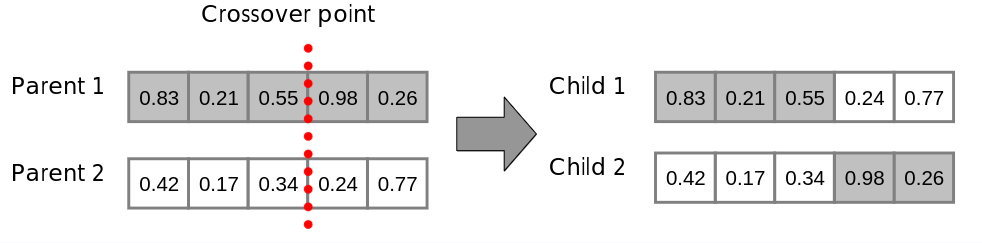
\includegraphics[width=0.6\textwidth]{imagenes/one-point-crossover.png}
    \end{center}
    \caption[One point crossover]{One-point crossover~\cite{purduelecture}}
\end{figure}

\subsubsection{Cruce continuo}
\textbf{Blend crossover}: Dado dos números reales para cada uno de los genes de los padres al hijo se le asignará un número aleatorio entre ese rango de gen para cada gen que conforme al vector cromosómico~\cite{purduelecture}.
\begin{figure}[htp]
    \begin{center}
        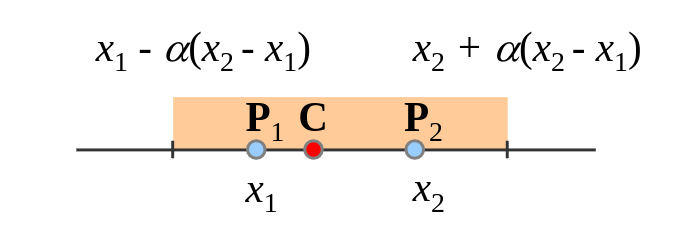
\includegraphics[width=0.6\textwidth]{imagenes/blend-crossover.png}
    \end{center}
    \caption[Blend crossover]{Blend crossover~\cite{purduelecture}}
\end{figure}

\subsubsection{Mutación binaria}
Su propósito es mantener la diversidad genética de los cromosomas de una población de un algoritmo evolutivo.
El operador más básico y clásico consiste en cambiar un bit arbitrario de un genotipo o solución de un algoritmo genético binario a su estado inverso dada una probabilidad de mutación~\cite{mirjalili2019genetic}.

\subsubsection{Mutación continua}
Esta mutación se utiliza especialmente en problemas en los que se busca una exploración más amplia del espacio de búsqueda, ya que la distribución de Cauchy tiene colas pesadas y puede generar valores alejados del centro con mayor probabilidad en comparación con una distribución normal:
\begin{equation}
    m(x_i) =
    \begin{cases}
        (2r)^{\frac{1}{\eta+1}}-1 & \text{if p $\leq 0.5$} \\
        1-(2r)^{\frac{1}{\eta+1}} & \text{if p $> 0.5$}    \\
    \end{cases}
\end{equation}
Esta función de mutación está diseñada para generar una exploración más amplia del espacio de búsqueda, con la posibilidad de generar valores más alejados del centro de la distribución. La variable $r$ es un número a aleatorio y $\eta$ es una variable de control.

\subsubsection{Elitismo}
El elitismo garantiza que las soluciones de alta calidad sobrevivan en las generaciones futuras, ayudando en la explotación del espacio de búsqueda. La cantidad de individuos élite seleccionados debe ser elegida con precisión~\cite{mirjalili2019genetic}.

\section{Algoritmos de colonias de hormigas}
\subsection{Introducción}
El algoritmo de colonia de hormigas o \textbf{ACO} es una técnica probabilística que trata de resolver problemas computacionales que pueden ser reducidos a la búsqueda de caminos óptimos a través de grafos. Se basa en el comportamiento de las hormigas reales y su comunicación vía feromonas. Las hormigas vagan por el mundo en búsqueda de comida de forma aleatoria. Cuando estas encuentran comida, dejan trazas de feromonas en su camino, de esta forma, si otras hormigas encuentran ese rastro, se hace más probable que recorran ese camino y dejen de vagar de forma aleatoria. Sin embargo, las trazas de feromonas se evaporan con el tiempo, perdiendo su fuerza de atracción sobre otras hormigas. De esta forma, si el camino es muy largo, la hormiga tardará mucho en recorrerlo y la traza de feromonas tendrá más tiempo a evaporarse. De manera análoga, a más corto es el camino, más rápido se recorre y más densidad de feromonas acumula~\cite{kashef_advanced_2015}.

\subsection{Funcionamiento y Operadores}
Para poder adaptar el algoritmo ACO a un problema es necesario reducir ese problema a la búsqueda del camino más corto dentro de un grafo ponderado. De esta forma, la \textbf{representación} en este tipo de algoritmo debe ser la de un grafo.
Cada característica del problema original se representa como un nodo $n$. Los caminos que conectan a los nodos ($e$) representan la elección del subconjunto de características. El camino deberá ser lo más corto posible maximizando a su vez el \textbf{accuracy}~\cite{kashef_advanced_2015}.

\subsubsection{Regla de transición probabilística}
\begin{equation}
    P_{ij}^k(t)=\begin{cases} \frac{\tau_{ij}^{\alpha}\eta_{ij}^{\beta}}{\sum_l\tau_{il}^{\alpha}\eta_{il}^{\beta}} & \text{Si $l$ y $k$ son nodos admisibles} \\ 0 & \text{De lo contrario} \end{cases}
\end{equation}
Donde:
\begin{itemize}
    \item $P_{ij}^k(t)$ denota la probabilidad de transición de un nodo de $i$ a $j$ en la $k$-hormiga (agente) en el instante de tiempo $t$.
    \item $\tau_{ij}$ es la cantidad de traza de feromona en la arista $(i,j)$ en el momento $t$. $\eta_{ij}$ es la heurística de deseabilidad o visibilidad de la arista.
    \item $\beta$ y $\alpha$ son dos parámetros que controlan la importancia relativa del valor de la feromona vs la información de la heurística.
\end{itemize}

\subsubsection{Evaporación de feromona}
Después de que todas las hormigas hayan terminado su camino, la evaporación de feromonas comienza. El contenido de feromonas del camino $(i,j)$ en el instante $t+1$ es:
\begin{equation}
    \tau_{ij}(\text{new})=(1-p)\tau_{ij}(t)+\sum_{k=1}^m\Delta\tau_{ij}^k(t)+\Delta\tau_{ij}^g(t)
\end{equation}
Donde:
\begin{itemize}
    \item $\Delta\tau_{ij}^k=\begin{cases}\frac{Q}{F^k}&\hspace{6mm}\text{Si la hormiga k pasa por la arista (i,j) en }T^k\\0 &\hspace{6mm}\text{De lo contrario}\end{cases}$
    \item $p\in (0,1]$ es el ritmo de evaporación.
    \item $m$ es el número de hormigas.
    \item $\Delta\tau_{ij}^k$ y $\Delta\tau_{ij}^g$ son respectivamente, la cantidad de feromonas colocadas en la arista $(i,j)$ por la hormiga $k$ y la cantidad de feromonas depositadas por la mejor hormiga $g$ en el instante $t$ sobre la arista $(i,j)$.
    \item $Q$ es una constante y $F^k$ es el valor de coste de la solución encontrada por la hormiga $k$ en el tour $T^k$, es decir, $F^k$ es el \textit{fitness} de la hormiga $k$.
\end{itemize}
Se utiliza el sistema \textit{max-min}, solo la mejor hormiga puede depositar feromona.\\[6pt]
En el algoritmo original, no había heurística de deseabilidad o visibilidad ($\eta$), solo información en términos de feromona~\cite{dorigo_ant_1999}.

\section{Optimización por enjambre de partículas}
\subsection{Introducción}
El algoritmo conocido como optimización por enjambre de partículas o en inglés \textit{particle swarm optimization} fue concebido en $1995$ por James Kennedy y Russel Eberhart~\cite{kennedy_particle_1995}. En este algoritmo, un conjunto de soluciones candidatas, llamadas partículas, se mueven en un espacio de búsqueda multidimensional. Cada partícula ajusta su posición de acuerdo con su experiencia personal y la experiencia del grupo.\\[6pt]
Para la versión binaria se utilizan funciones de transferencia.

\subsection{Funcionamiento y Operadores}
Las soluciones son descritas como individuos dentro de un enjambre (conjunto total de posibles soluciones) que tienen una posición y una velocidad en todo momento. La posición de estos individuos representa la solución en sí.

\subsubsection{Velocidad}
\begin{equation}
    v_{i}(t+1) = v_{i}(t) + c_1 \cdot \text{rand}() \cdot (pbest_{i} - x_{i}(t))+ c_2 \cdot \text{rand}() \cdot (gbest - x_{i}(t))
\end{equation}

Donde:
\begin{itemize}
    \item $v_{i}(t+1)$ es la velocidad de la partícula $i$ en la siguiente iteración.
    \item $v_{i}(t)$ es la velocidad de la partícula $i$ en la iteración actual.
    \item $c_1$ y $c_2$ son factores de aceleración que controlan la influencia de las mejores posiciones.
    \item $\text{rand}()$ es un número aleatorio en el rango [0, 1].
    \item $pbest_{i}$ es la mejor posición histórica de la partícula $i$.
    \item $x_{i}(t)$ es la posición actual de la partícula $i$ en la iteración $t$.
    \item $gbest$ es la mejor posición global del grupo.
\end{itemize}

\subsubsection{Posición}

\begin{equation}
    x_{i}(t+1) = x_{i}(t) + v_{i}(t+1)
\end{equation}

Estas ecuaciones se utilizan para guiar el movimiento de las partículas a través del espacio de búsqueda hacia las mejores soluciones, adaptándose tanto a la mejor solución encontrada por la propia partícula ($pbest$) como a la mejor solución encontrada por cualquier partícula en el enjambre ($gbest$)~\cite{kennedy_particle_1995}. Con el tiempo, las partículas tienden a converger hacia las mejores soluciones conocidas.

\section{Evolución diferencial}
La evolución diferencial surgió como un algoritmo de optimización para problemas no diferenciables y no lineales, con pocas variables de control, robusto, paralelizable y muy eficaz. El algoritmo de evolución diferencial o \textit{differential evolution} en inglés fue diseñado para resolver problemas continuos, a diferencia del propósito original de su ``hermano gemelo'' el algoritmo genético, cuya finalidad inicial era resolver problemas binarios. Este algoritmo fue presentado en $1996$ por Storn y Price en \cite{storn_differential_1997}.\\[6pt]
En la evolución diferencial, la diferencia de vectores es un concepto clave que se utiliza en el operador de mutación. Esta se calcula restando dos vectores de la población. Gracias a esta operación puede calcularse la distancia entre vectores y esto conlleva una serie de ventajas~\cite{storn_differential_1997}:
\begin{itemize}
    \item Las posiciones de los individuos proporcionan información ya que si los individuos están bien distribuidos (y si la población es lo suficientemente grande), la población inicial será una buena representación de todo el espacio de búsqueda.
    \item Las distancias entre estos individuos serán inversamente proporcionales al tamaño de la población.
    \item A medida que avanza la búsqueda y los individuos comienzan a converger hacia un óptimo local, las distancias entre los individuos comenzarán a disminuir.
\end{itemize}
Para la versión binaria se utilizan funciones de transferencia.

\subsection{Funcionamiento y Operadores}
La representación suele ser la misma que en otros algoritmos metaheurísticos. DE fue diseñado para optimizar un problema continuo, por lo que la población debería ser un conjunto de números reales.

\subsubsection{Mutación}
La operación de mutación produce un vector, conocido como vector de prueba o en inglés \textit{trial vector}. Para ello se hace uso de un vector objetivo y una diferencia de vectores ponderada. La mutación elige a un padre $x_{i}$, generando un vector de prueba $u_{i}$ siguiendo lo siguientes pasos:
\begin{enumerate}
    \item Se selecciona un vector objetivo $x_{i_1}$ tal que $i\neq i_1$.
    \item Se selecciona aleatoriamente dos individuos $x_{i_2}$ y $x_{i_3}$ de la población tal que $i\neq i_1\neq i_2\neq i_3$ y $i_2,i_3$ sean seleccionados con una probabilidad uniforme. Es necesario que todos los individuos tengan la misma probabilidad de selección.
\end{enumerate}
Finalmente, se calcula el vector de prueba:
\begin{equation}
    u_i = x_{i_1}+\beta\dot(x_{i_2}-x_{i3})
\end{equation}
Donde $\beta$ es un factor de escalado que controla la amplificación de la variación diferencial (mutación más diversa/grande)~\cite{storn_differential_1997}.

\begin{figure}[htp]
    \begin{center}
        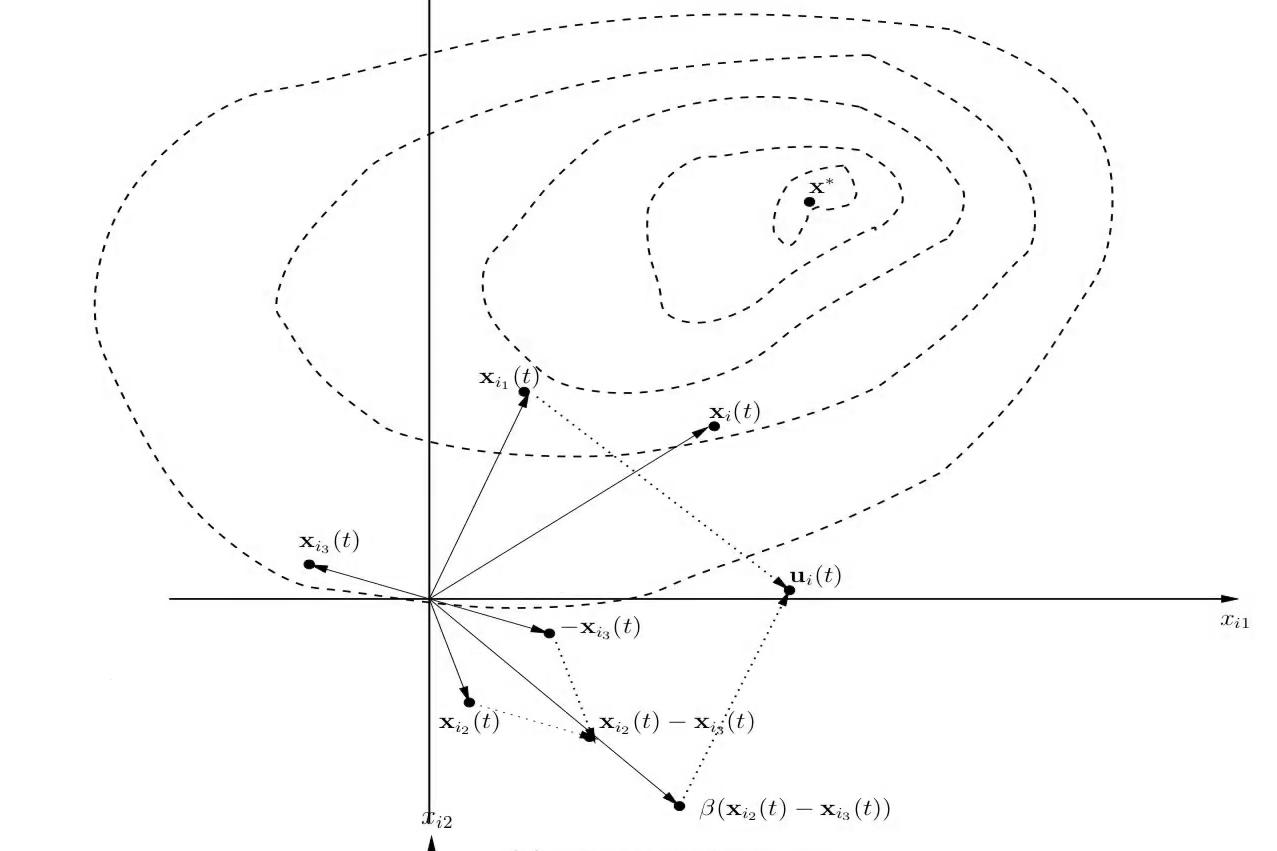
\includegraphics[width=1\textwidth]{imagenes/de-mutation.png}
    \end{center}
    \caption[Mutación en DE]{Esta figura ha sido seleccionada de \cite{10.5555/1557464}. Muestra de manera gráfica en un espacio bidimensional como funciona el operador de mutación y cómo se crea el ``trial vector''.}
\end{figure}

Una ventaja del uso de diferencias de vectores en la mutación es que ayuda a mantener la forma de la distribución en lugar de centrarse en el centro, como hacen muchos operadores de cruce. Además, al tener una media de la distribución cercana a cero, se minimiza la deriva genética~\cite{10.5555/1557464}. Este fenómeno puede causar cambios en la composición genética de la población a lo largo de las generaciones, especialmente en poblaciones pequeñas. Por lo tanto, mantener una media cercana a cero ayuda a prevenir sesgos en la deriva genética.

\subsubsection{Cruce}
El cruce implementa una recombinación del vector de prueba $u_i$ y el vector padre $x_i$ para producir un vector hijo $x^\prime_i$.
\begin{equation}
    x^\prime_{ij}=\begin{cases} u_{ij} & \text{Si $j\in \mathcal{J}$} \\ x_{ij} & \text{De lo contrario} \end{cases}
\end{equation}
Donde $\mathcal{J}$ es un conjunto de puntos de perturbación. Estos índices pueden ser calculados de muchas formas, por ejemplo, de manera aleatoria.

\begin{figure}[htp]
    \begin{center}
        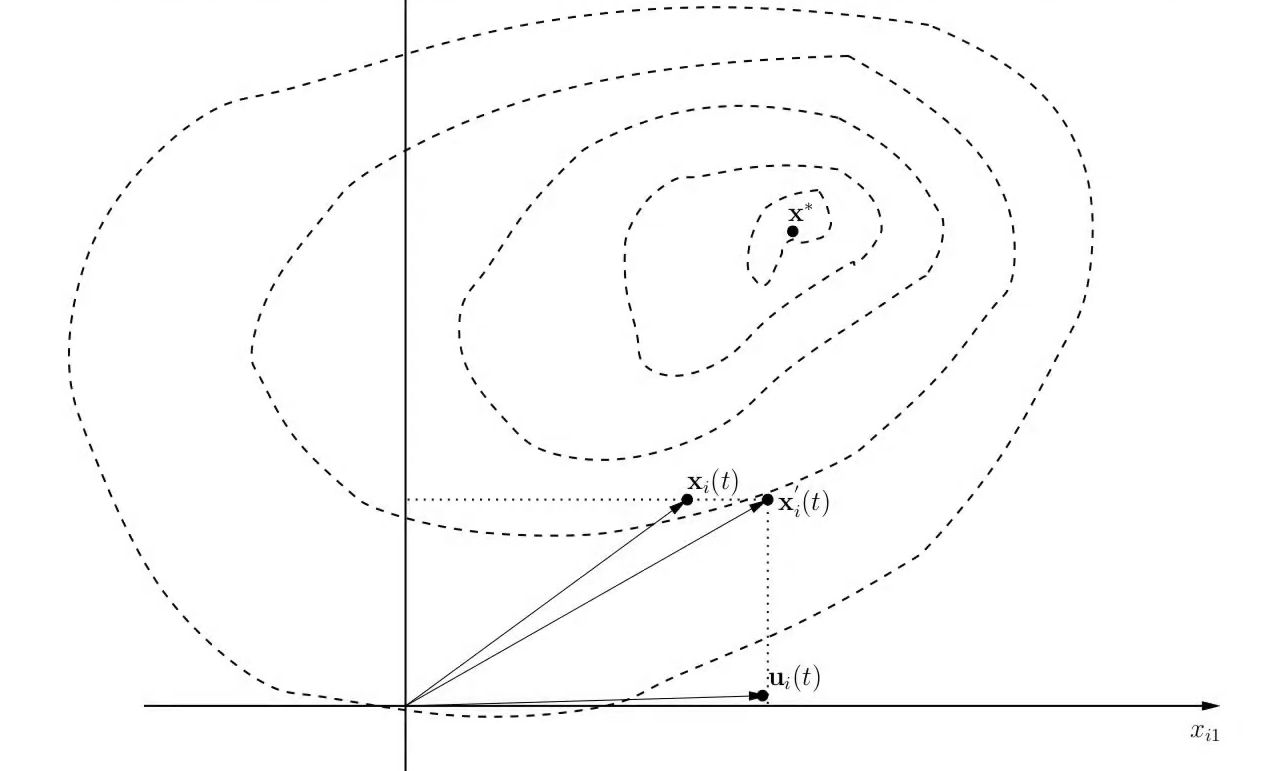
\includegraphics[width=1\textwidth]{imagenes/de-crossover.png}
    \end{center}
    \caption[Crossover en DE]{Esta figura ha sido seleccionada de \cite{10.5555/1557464}. Muestra de manera gráfica en un espacio bidimensional como funciona el operador de cruce al recombinar los genes/características de los vectores padre y ``trial''.}
\end{figure}

\subsubsection{Selección}
Si el vector hijo, al evaluarlo, tiene un valor \textit{fitness} mejor que el vector padre, entonces se sustituye el vector $x_i$ por el vector $x^\prime_i$. De otra forma, el vector padre continuará en la población para la siguiente generación~\cite{storn_differential_1997}.

\section{Optimización por colonia de abejas artificial}
\subsection{Introducción}
El algoritmo del enjambre de abejas artificial es un algoritmo estocástico evolutivo, al igual que los ya mencionados anteriormente, que se basa en el comportamientos de los enjambres de abejas para la optimización de problemas. El modelo usado en este algoritmo depende de tres factores, las fuentes de alimento, las abejas buscadores empleadas y las abejas buscadoras libres (hay dos tipos)~\cite{karaboga_idea_nodate}.\\[6pt]
Para la versión binaria se utilizan funciones de transferencia.

\subsection{Funcionamiento y Operadores}
Los operadores del algoritmo son los siguientes:
\begin{enumerate}
    \item \textbf{Abejas Empleadas (Employed Bees)}: Estas abejas están asociadas con fuentes de alimento específicas y son responsables de explotar estas fuentes. Llevan información sobre la fuente de alimento, incluyendo la distancia, la dirección y la rentabilidad, y comparten esta información dentro de la colmena, influyendo en las decisiones de otras abejas.

    \item \textbf{Abejas Observadoras (Outlooker Bees)}: Estas abejas esperan dentro de la colmena y toman decisiones sobre a qué fuentes de alimento dirigirse basándose en la información proporcionada por las abejas empleadas. Seleccionan las fuentes de alimento según la probabilidad que está directamente relacionada con la rentabilidad de las fuentes.

    \item \textbf{Abejas Exploradoras (Scout Bees)}: Son abejas que buscan nuevas fuentes de alimento sin información previa. Su rol es crucial para la exploración y el descubrimiento de nuevas fuentes de alimento. Cuando una fuente se agota o no mejora después de cierto número de intentos (determinado por un parámetro de control llamado "límite"), una abeja empleada puede convertirse en exploradora.
\end{enumerate}

\begin{figure}[htp]
    \centering
    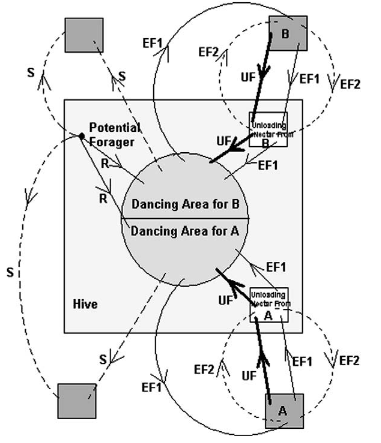
\includegraphics[width=0.9\textwidth]{imagenes/abco.png}
    \caption[Comportamiento de ABCO]{Figura obtenida de~\cite{Karaboga2009108}.}
\end{figure}

Estos operadores trabajan en un ciclo repetitivo donde las abejas empleadas primero van a las fuentes de alimento y actualizan la información sobre su rentabilidad. Luego, las abejas observadoras seleccionan fuentes de alimento basadas en esta información actualizada y las abejas exploradoras buscan nuevas fuentes~\cite{karaboga_idea_nodate}. Este proceso se repite hasta cumplir con los criterios de terminación del algoritmo.

\section{Algoritmo de optimización del saltamontes}
\subsection{Introducción}
Los \textbf{grasshoppers} (saltamontes o langosta cuando están en enjambre) son insectos cuyo ciclo de vida consiste en tres etapas: \textit{huevo, ninfa, adulto}. Un saltamontes puede ser encontrado en el enjambre en su estado ninfa y adulto. La diferencia entre ninfa y adulto es la velocidad de movimiento con pasos pequeños en la ninfa y lo contrario en su vida adulta (Las soluciones adultas se encargan de la exploración y las ninfas de la explotación)~\cite{saremi_grasshopper_2017}.\\[6pt]
Para la versión binaria se utilizan funciones de transferencia.
\subsection{Funcionamiento y Operadores}
\subsubsection{Operador de posición (primera propuesta)}
La posición de un individuo se define en la siguiente ecuación:
\begin{equation}
    x_i = r_1s_1+r_2g_i+r_3a_i
\end{equation}
Donde $x_i$ es la posición del agente número $i$, $s$ la interacción social, $g$ la fuerza gravitacional, $a$ la advección del viento y $r_1, r_2, r_3$ son números aleatorios entre $[0,1]$.
Esta función de actualización de posición no puede ser usada para la optimización debido a que se alcanza la zona de comfort de manera prematura y no se converge en un punto específico~\cite{saremi_grasshopper_2017}.

\subsubsection{Posición (propuesta final)}

\begin{equation}
    X_i^d=c_1\left(\sum_{j=1,j\neq i}^N c_2\frac{ub_d-lb_d}{2}s(|x_j^d-x_i^d|)\frac{x_j-x_i}{d_{ij}}\right)+\hat{T_d}
    \label{eq:goa-position}
\end{equation}

Donde $ud_b$ es la cota superior en la dimensión $D$, $lb_d$ es la cota inferior en la dimensión $D$, $\hat{T_d}$ es el valor de la dimensión $D$ en el objetivo (la mejor solución encontrada hasta la fecha) y $c$ es el coeficiente decreciente para hacer cada vez más pequeña la zona de comfort, zona de atracción y zona de repulsión.

No se considera la gravedad (G) y la dirección del viento siempre es a favor del objetivo $\hat{T_d}$.

Una diferencia con otros algoritmos de enjambres como PSO es que \textbf{GAO} actualiza la posición de cada saltamontes a partir de la posición actual, el mejor punto encontrado hasta el momento y la posición de todos los otros agentes, mientras que \textbf{PSO} lo hace a partir de la posición actual del agente y la mejor posición encontrada~\cite{saremi_grasshopper_2017}.

Esto significa que PSO no tienen en cuenta al resto de agentes, mientras que GAO sí.

Los parámetros $c_1, c_2$ tienen dos propósitos:
\begin{itemize}
    \item $c_1$ $\rightarrow$ Reduce el movimiento del enjambre entero alrededor del objetivo, es decir, maneja la relación entre exploración y explotación para el conjunto global de soluciones.
    \item $c_2$ $\rightarrow$ Reduce la zona de comfort y las regiones de repulsión y atracción. $s$ es la función que decide si un agente debe sentirse atraído o repelido al objetivo, mientras que $\frac{ub_d-lb_d}{2}$ decrece de manera lineal el espacio de búsqueda a medida que $c_2$ decrece.
\end{itemize}

Ha de tenerse en cuenta también que en el proceso de búsqueda, la exploración debe ir antes que la explotación. En los saltamontes sin embargo, la fase explotativa que es la \textbf{ninfa} es la que se da primero. Por ello el parámetro $c$ debe decrecer a medida que las iteraciones sobre el algoritmo van pasando. Este mecanismo hace que se promueva la explotación a medida que las iteraciones se incrementan, ya que se va reduciendo cada vez más el movimiento general del enjambre y se reduce la zona de comfort. $c$ se actualiza por tanto así:
\begin{equation}
    c = c_{\text{max}} - l \cdot \frac{c_{\text{max}} - c_{\text{min}}}{L}
\end{equation}

Donde $l$ es la iteración actual y $L$ el número máximo de iteraciones.

\begin{figure}[htp]
    \begin{center}
        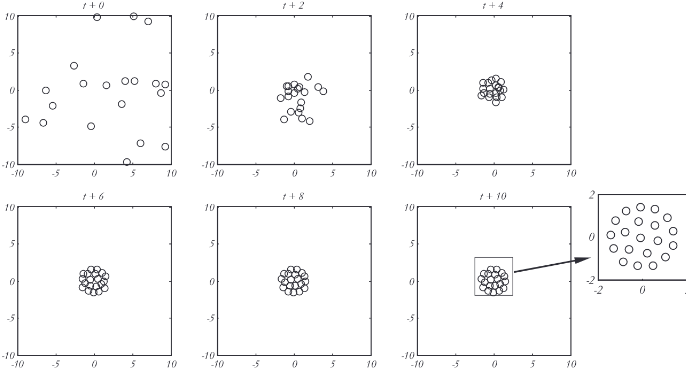
\includegraphics[width=0.8\textwidth]{imagenes/goa-position-convergence.png}
    \end{center}
    \caption[Convergencia en GOA]{Esta figura ha sido seleccionada de \cite{saremi_grasshopper_2017}. Muestra la convergencia de los ``saltamontes'' en tan solo unas pocas iteraciones usando la fórmula \ref{eq:goa-position}.}
\end{figure}

\section{Algoritmo de la libélula}
\subsection{Introducción}
Los \textbf{dragonflies} (libélulas en español) son pequeños insectos que se pueden ver en enjambre solo cuando cazan o migran, dando lugar a dos tipos de enjambre:
\begin{itemize}
    \item Las diferencias dadas entre ambos enjambres son notorias. En caza, se organizan en enjambres pequeños que vuelan en muchas direcciones en busca de comida. Este tipo de enjambre es llamado \textbf{estático}. Cuando se organizan en enjambres para migrar, estos son numerosos y vuelan en una sola dirección. Estos enjambres en contraposición a los anteriores son llamados \textbf{dinámicos}~\cite{mirjalili_dragonfly_2016}.
    \item Es obvio el paralelismo que se da entre las principales fases de la búsqueda optimizatoria (\textbf{exploración y explotación}). La fase dinámica es un paralelismo con la exploración, ya que se buscan pequeños objetivos en grupos por el espacio. La fase estática (explotación) se da cuando todos los agentes empiezan a migrar a una dirección concreta.
\end{itemize}
Para la versión binaria se utilizan funciones de transferencia.

\subsection{Funcionamiento y Operadores}

\subsubsection{Separación}
\begin{equation}
    S_i = -\sum_{j=1}^N X - X_j
\end{equation}
Se refiere a la elusión estática de colisión entre individuos con su vecindario. Donde $X$ es la posición del agente actual y $X_j$ la posición de su vecino número $j$. Mientras que $N$ es el número total de agentes.

\subsubsection{Alineamiento}
\begin{equation}
    A_i = \frac{\sum_{j=1}^N V_i}{N}
\end{equation}
Se refiere a la coordinación de velocidad entre individuos de un vecindario. Donde $V_j$ es la velocidad del individuo número $j$ en el vecindario.

\subsubsection{Cohesión}
\begin{equation}
    C_i = \frac{\sum_{j=1}^N X_j}{N} - X
\end{equation}
Se refiere a la fuerza de atracción de los individuos hacia el centro de masa del vecindario. Se da por hecho un radio alrededor de cada libélula agrupando su vecindario, pues este es muy importante para el comportamiento de esta. En un enjambre dinámico, las libélulas tienden a alinear su vuelo al tiempo que mantienen una separación y cohesión adecuadas.\\[6pt]
En un enjambre estático, sin embargo, las alineaciones son muy bajas mientras que la cohesión es alta para atacar a las presas. Por lo tanto, se asigna a las libélulas pesos de alta alineación y baja cohesión cuando exploran el espacio de búsqueda y de baja alineación y alta cohesión cuando explotan el espacio de búsqueda. Para la transición entre exploración y explotación, los radios de vecindad se incrementan proporcionalmente al número de iteraciones~\cite{mirjalili_dragonfly_2016}.
\begin{figure}[htp]
    \centering
    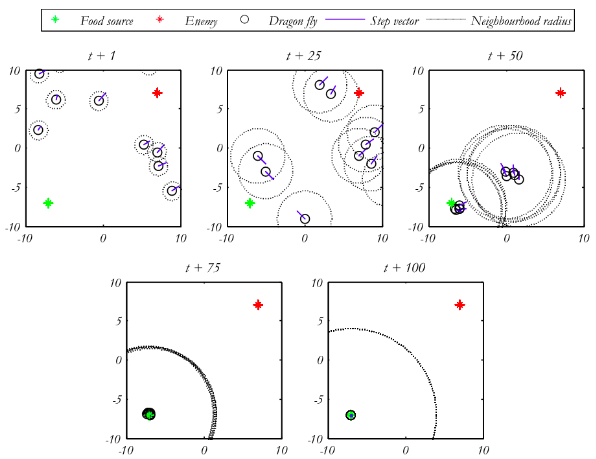
\includegraphics[width=0.9\textwidth]{imagenes/da-operators.png}
    \caption[Vecindario de libélulas]{Vecindario de libélulas~\cite{mirjalili_dragonfly_2016}.}
\end{figure}

\subsubsection{Atracción comida}
\begin{equation}
    F_i = X^+ - X
\end{equation}
La fuerza de atracción hacia la comida (la mejor posición encontrada hasta el momento). Donde $X^+$ es la mejor posición encontrada hasta el momento.

\subsubsection{Repulsión depredador}
\begin{equation}
    E_i = X^- + X
\end{equation}
La fuerza de repulsión hacia un depredador (la peor posición encontrada hasta el momento). Donde $X^-$ es la peor posición encontrada hasta el momento.

\subsubsection{Dirección}
\begin{equation}
    \Delta X_{t+1} = (sS_i + aA_i + cC_i + fF_i + eE_i) + w\Delta X_t
\end{equation}
El delta de $X$ indica el vector dirección del movimiento de las libélulas. Cada elemento en minúscula es el factor del operador al que multiplica, de forma que es posible acentuar el efecto de cada uno de estos con múltiples combinaciones.

\subsubsection{Posición}
\begin{equation}
    X_{t+1} = X_{t} + \Delta X_{t+1}
\end{equation}
El operador de actualización de posición.

\section{Algoritmo de optimización de ballenas}
\subsection{Introducción}
Simula el comportamiento de las ballenas jorobadas en la caza, utilizando tanto el azar como el mejor agente de búsqueda para perseguir a la presa. Además, emplea una espiral para simular el mecanismo de ataque de la red de burbujas de las ballenas jorobadas~\cite{mirjalili_whale_2016}.\\[6pt]
Para la versión binaria se utilizan funciones de transferencia.

\subsection{Funcionamiento y Operadores}
\subsubsection{Rodeado de presa}
\begin{equation}
    \vec{D}=|\vec{C}\cdot\vec{X}^*(t)-\vec{X}(t)|
\end{equation}
\begin{equation}
    \vec{X}(t+1)=\vec{X}^*(t)-\vec{A}\cdot\vec{D}
\end{equation}
Donde $t$ indica la iteración actual, $\vec{A}$ y $\vec{C}$ son vectores de coeficientes, $X^*$ es el vector de posición de la mejor solución encontrada hasta el momento y $\vec{X}$ es el vector posición.

Los vectores $\vec{A}$ y $\vec{C}$ se calculan como sigue:
\begin{equation}
    \vec{A}=2\vec{a}\cdot\vec{r}-\vec{a}
\end{equation}
\begin{equation}
    \vec{C}=2\cdot\vec{r}
\end{equation}
Donde $\vec{a}$ es decrementado linealmente desde $2$ hasta $0$ y $\vec{r}$ es un vector aleatorio con valores en $[0,1]$.

\subsubsection{Ataque de red de burbujas (explotación)}
\begin{itemize}
    \item \textbf{Mecanismo de encogimiento del cerco}
          Este mecanismo es conseguido mediante el decremento del valor de $\vec{a}$. El vector $\vec{A}$ es un vector de valores aleatorios en el intervalo $[-a,a]$ donde $a$ es decrementado desde $2$ hasta $0$.
          \begin{figure}[htp]
              \centering
              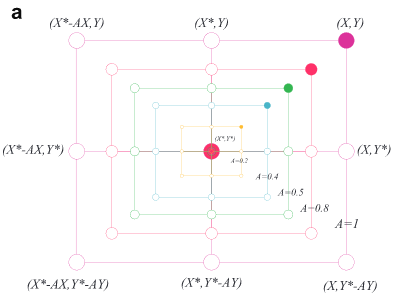
\includegraphics[width=0.5\textwidth]{imagenes/wao-shrinking-circle-prey-mechanism.png}
              \caption[Mecanismo de encogimiento del cerco]{Ataque de red de burbujas usando el mecanismo de encogimiento del cerco~\cite{mirjalili_whale_2016}.}
          \end{figure}

    \item \textbf{Mecanismo de actualización de posición en espiral}
          Este mecanismo calcula la distancia entre la ballena $(x,y)$ y la presa $(x^*, y^*)$. Una ecuación con forma de espiral es creada entonces entre la ballena y la presa para simular el comportamiento de estas al cazar.
          \begin{figure}[htp]
              \centering
              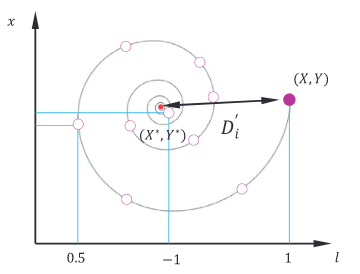
\includegraphics[width=0.5\textwidth]{imagenes/spiral-update-position-wao.png}
              \caption[Mecanismo de actualización de posición en espiral]{Ataque de red de burbujas usando el mecanismo de actualización de posición en espiral~\cite{mirjalili_whale_2016}.}
          \end{figure}

          \begin{equation}
              \vec{X}(t+1)=\vec{D}^{'}\cdot e^{bl}\cdot cos(2\pi l)+\vec{X}^*(t)
          \end{equation}
          Donde $\vec{D}^{'}=|\vec{X}^*(t)-\vec{X}(t)|$ e indica la distancia entre presa y ballena. $b$ es una constante para definir la forma de la espiral, $l$ es un número aleatorio entre $[-1,1]$.
\end{itemize}

Se utilizan ambos mecanismos, dependiendo de si cierto número $p$ aleatorio es mayor o menor a $0.5$.

\subsubsection{Búsqueda de la presa (exploración)}
El mismo método utilizando el vector $\vec{A}$ puede ser utilizado para la exploración. Se puede usar $\vec{A}$ con valores más grandes a $1$ o menores a $-1$ para forzar al agente a moverse lejos de otro agente.
\begin{equation}
    \vec{D}=|\vec{C}\cdot\vec{X}_{rand}-\vec{X}|
\end{equation}
\begin{equation}
    \vec{X}(t+1)=\vec{X}_{rand}-\vec{A}\cdot\vec{D}
\end{equation}
Cuando $|A|\geq 1$ $\rightarrow$ Exploración, cuando $|A|<1$ $\rightarrow$ Explotación.

\section{Algoritmo del murciélago}
\subsection{Introducción}
El algoritmo \textit{metaheurístico} de los murciélagos se basa en la capacidad de eco-localización de estos para detectar a su presa y cazarla finalmente. La eco-localización de los murciélagos no solo les permite detectar a su presa, si no discriminar entre distintos tipos de insectos. Más concretamente, este algoritmo se basa en los micro murciélagos, pues estos usan más frecuentemente la eco-localización en comparación a otras especies de murciélagos. Estos murciélagos emiten un pulso de sonido, el cual, rebota en los objetos y entidades cercanas, permitiendo al murciélago componer una ``visión'' general de sus alrededores. La frecuencia del pulso emitido podría estar relacionada con distintas estrategias de caza~\cite{yang_new_2010}.
\subsubsection{Acústica de la eco-localización}
Aunque cada pulso dura solo unos pocos milisegundos (entre 8 y 10 ms), mantiene una frecuencia constante, generalmente entre 25 kHz y 150 kHz. La longitud de onda ($\lambda$) de estos impulsos ultrasónicos, con una frecuencia ($f$) y velocidad del sonido ($v$) en el aire a 340 m/s, está dada por
\begin{equation}
    \lambda = \frac{v}{f}
\end{equation}
con longitudes entre 2 mm y 14 mm para frecuencias de 25 kHz a 150 kHz, respectivamente. Esta longitud de onda coincide con el tamaño de las presas. Los murciélagos pueden detectar obstáculos tan pequeños como cabellos humanos, utilizando la eco-localización para construir un modelo 3D del entorno, y discriminando distancias, orientaciones y tipos de presas. Aunque los murciélagos tienen buena vista y olfato, utilizan principalmente la eco-localización para la detección de presas y la navegación eficiente~\cite{yang_new_2010}.\\[6pt]
Para la versión binaria se utilizan funciones de transferencia.
\subsection{Funcionamiento y Operadores}
Para simplificar:
\begin{itemize}
    \item Los murciélagos usan la ecolocación para percibir la distancia y distinguir alimento de barreras.
    \item Vuelan aleatoriamente con velocidad $v_i$ y frecuencia fija $f_{min}$, ajustando longitud de onda $\lambda$ y sonido $A_0$.
    \item Se asume que la intensidad del sonido varía desde $A_0$ hasta un mínimo $A_{min}$.
\end{itemize}
\subsubsection{Movimiento}

Las soluciones (posiciones) y las velocidades de los murciélagos en un instante $i$ son:
\begin{equation}
    \begin{aligned}
         & x_i^t = x_i^{t-1} + v_i^t                                      \\
         & v_i^t = v_i^{t-1} + (x_i^t - x_*) f_i                          \\
         & f_i = f_{\text{min}} + (f_{\text{max}} - f_{\text{min}}) \beta
    \end{aligned}
\end{equation}
Donde $\beta$ es un vector aleatorio escogido de una distribución uniforme, $x_*$ es la mejor posición global que es seleccionada tras comprobar los $n$ murciélagos. Como el productor de $\lambda_i f_i$ es el incremento de la velocidad, se puede usar tanto uno como otro para ajustar la velocidad mientras el otro es fijado, todo depende del problema de interés~\cite{yang_new_2010}. En el documento original, se utiliza un rango para $f$ de $[0,100]$. A cada murciélago se le asigna una frecuencia uniformemente de $[f_{\text{min}},f_{\text{max}}]$. Una vez se ha seleccionado una mejor solución, se actualizan los vectores posición de cada murciélago:
\begin{equation}
    x_{\text{new}} = x_{\text{old}} + \epsilon A^t
\end{equation}
Donde $\epsilon \in [-1,1]$ es un número aleatorio y $A^t$ es la intensidad sonora media de los murciélagos.

\subsubsection{Intensidad sonora y Emisión de pulso}

La intensidad sonora y el ratio de emisión de pulsos deben actualizarse según avance el número de iteraciones. $A_i$ debe decrementarse a la vez que el ratio $r_i$ se incrementa según el murciélago se acerca a su presa~\cite{yang_new_2010}. Se actualizan del siguiente modo:
\begin{equation}
    \begin{aligned}
         & A_i^{t+1} = \alpha A_i^t, \quad r_i^{t+1} = r_i^0 [1 - \exp(-\gamma t)]
    \end{aligned}
\end{equation}
Donde $\gamma, \alpha$ son constantes. Estos valores solo se actualizan si las nuevas soluciones son mejores, de manera que se guíe hacia un óptimo.

\section{Optimización de los lobos grises}
\subsection{Introducción}

\begin{itemize}
    \item El algoritmo se inspira en el comportamiento de la manada de los lobos grises y sus escala jerárquica. Los lobos grises son super-depredadores, es decir, están en la cima de la cadena alimentaria~\cite{mirjalili_grey_2014}. Su escala jerárquica es la siguiente:
          \begin{enumerate}
              \item $\alpha\rightarrow$ Los lobos alfa son aquellos que lideran la manada, no por su fuerza, si no por su capacidad organizativa dentro de la manada. Estos solo puede procrear dentro de la manada y son los encargados de tomar decisiones importantes sobre todo el conjunto.
              \item $\beta\rightarrow$ Los lobos beta son subordinados directos de los alfa. Son la opción más directa cuando se trata de sustituir a un alfa. Deben mostrar respeto a los alfa y comandan al resto de la manada según dicte el alfa.
              \item $\omega\rightarrow$ El nivel más bajo de la cadena. Son los últimos en comer, pero no por ello carecen de importancia, pues la manada puede llegar a enfrentarse a graves problemas cuando este nivel de lobos falta. Son totalmente necesarios para mantener la estructura.
              \item $\delta\rightarrow$ Lobos que someten a los omegas, pero que deben someterse a los alfas y omegas. A este grupo pertenecen los cazadores, ancianos, centinelas y cuidadores.
          \end{enumerate}

    \item Modelado de jerarquía:
          \begin{itemize}
              \item Se considera la solución más buena como la solución $\alpha$, siendo las siguientes en orden de mejor a peor \textbf{fitness} la $\beta$, la $\delta$ y por último la $\omega$.
              \item La caza (optimización) es guiada por las soluciones $\alpha$, $\beta$ y $\delta$ mientras que las soluciones $\omega$ siguen a estos tres lobos.
          \end{itemize}
\end{itemize}
Para la versión binaria se utilizan funciones de transferencia.

\subsection{Funcionamiento y Operadores}

\subsubsection{Rodeo de la presa}
\begin{equation}
    \vec{D}=|\vec{C}\cdot\vec{X}_p(t)-\vec{X}(t)|
\end{equation}
\begin{equation}
    \vec{X}(t+1)=\vec{X}_p(t)-\vec{A}\cdot\vec{D}
    \label{eq:grey-wolf-hunt}
\end{equation}
Donde $t$ indica la iteración actual, $\vec{A}$ y $\vec{C}$ son vectores de coeficientes, $\vec{X}_p$ es el vector posición de la presa y $\vec{X}$ el vector posición del lobo gris.
Los vectores $\vec{A}$ y $\vec{C}$ se calculan:
\begin{equation}
    \vec{A}=2\vec{a}\cdot\vec{r}_1-\vec{a}
\end{equation}
\begin{equation}
    \vec{C}=2\cdot\vec{r}_2
\end{equation}
Donde los componentes del vector $\vec{a}$ son decrementados de $2$ a $0$ linealmente según avanzan las iteraciones. Las variables  $r_1$ y $r_2$ son vectores aleatorios entre $[0,1]$.

\begin{figure}[htp]
    \begin{center}
        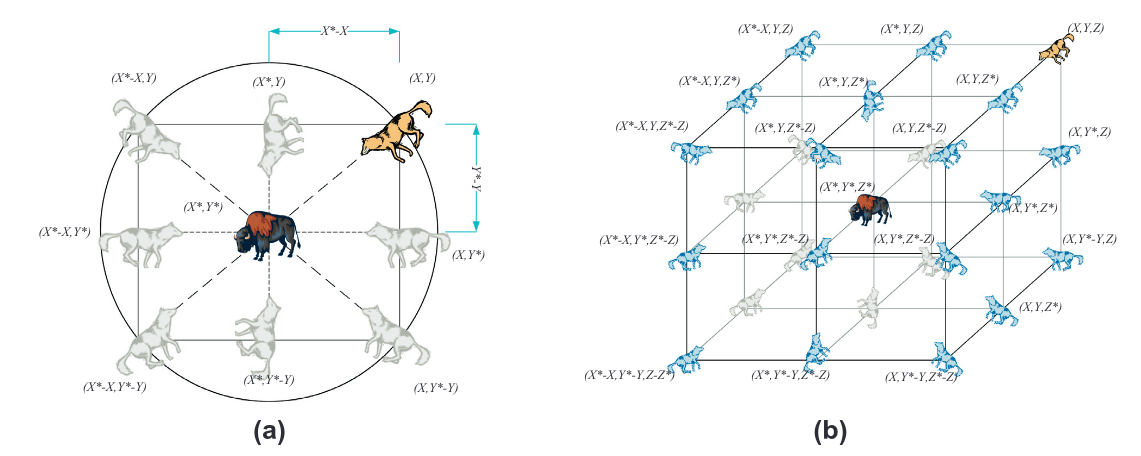
\includegraphics[width=1\textwidth]{imagenes/grey-wolf-hunt.png}
    \end{center}
    \caption[Rodeo de la presa en 2D y 3D]{Esta figura ha sido seleccionada de \cite{mirjalili_grey_2014}. Muestra en espacios 2D (a) y 3D (b) diferentes posiciones que un lobo puede tomar alrededor de la presa dada la ecuación \ref{eq:grey-wolf-hunt}. Define una vecindad alrededor de la solución en forma de hiper-esfera.}
\end{figure}

\subsubsection{Caza}
Se supone que el alfa, beta y delta tienen mayor conocimiento de donde está la presa (óptimo) y por tanto la posición del resto de lobos debe actualizarse siguiendo a estos tres primeros~\cite{mirjalili_grey_2014}.
\begin{equation}
    \vec{D}_{\alpha}=|\vec{C}_1\cdot\vec{X}_{\alpha}-\vec{X}|,\quad \vec{D}_{\beta}=|\vec{C}_2\cdot\vec{X}_{\beta}-\vec{X}|,\quad \vec{D}_{\delta}=|\vec{C}_3\cdot\vec{X}_{\delta}-\vec{X}|
\end{equation}
\begin{equation}
    \vec{X}_1=\vec{X}_{\alpha}-\vec{A}_1\cdot\vec{D}_{\alpha},\quad \vec{X}_2=\vec{X}_{\beta}-\vec{A}_2\cdot\vec{D}_{\beta},\quad \vec{X}_3=\vec{X}_{\delta}-\vec{A}_3\cdot\vec{D}_{\delta}
\end{equation}
\begin{equation}
    \vec{X}(t+1)=\frac{\vec{X}_1+\vec{X}_2+\vec{X}_3}{3}
\end{equation}

\subsubsection{Ataque a la presa (explotación)}
Cuando los lobos están muy cerca de la presa (solución óptima), el valor de $A$ disminuye, llevando a los lobos a converger hacia la presa. Esto se refleja en una reducción en la amplitud de los saltos en el espacio de búsqueda, facilitando una búsqueda local intensiva cerca de la mejor solución encontrada~\cite{mirjalili_grey_2014}.

\subsubsection{Búsqueda de la presa (exploración)}
Para fomentar la exploración y evitar los óptimos locales, los vectores $A$ pueden tomar valores que obliguen a los lobos a alejarse de la presa, explorando nuevas áreas del espacio de búsqueda. Este comportamiento se activa cuando los elementos de $A$ son mayores que $1$ o menores que $-1$, lo que amplía la capacidad del algoritmo para explorar el espacio de búsqueda de manera más amplia~\cite{mirjalili_grey_2014}.

\section{Algoritmo de la luciérnaga}
\subsection{Introducción}
Las luciérnagas son insectos capaces de producir un brillo único, muy visible y característico sobre todo de noche. El brillo que estas producen puede llegar a tener signficados que hoy dia siguen debatiendose en la comunidad científica. Pese a ello, se conoce que este brillo tiene dos funciones fundamentales y bien definidas:
\begin{enumerate}
    \item \textbf{Comunicación}: Sirve como instrumento para la comunicación entre dos luciérnagas para el apareamiento.
    \item \textbf{Atracción}: Se usa para atraer a potenciales presas de la luciérnaga.
\end{enumerate}
Por simplicidad del algoritmo, se asumen tres reglas sobre el comportamiento y naturaleza de las luciérnagas~\cite{yang_chapter_2014}:
\begin{enumerate}
    \item Las luciérnagas solo tienen un sexo, por lo que todas se ven atraídas por todas y no hay discriminación más allá de que una luciérnaga sea más atractica que otra.
    \item La luminosidad es proporcional a lo atractiva que es una luciérnaga para el resto.
    \item La luminosidad de una luciérnaga es determinada por los límites de la función objetivo.
\end{enumerate}
Para la versión binaria se utilizan funciones de transferencia.

\subsection{Funcionamiento y Operadores}
\subsubsection{Intensidad de la luz}
\begin{equation}
    \beta = \beta_0 e^{-\gamma r^2}
\end{equation}
Donde $\beta_0$ es el atractivo en $r=0$, es decir, en distancia igual a $0$ y $\gamma$ es un coeficiente fijo de absorción de luz~\cite{yang_chapter_2014}. La distancia entre dos luciérnagas es la distancia cartesiana:
\begin{equation}
    r_{ij}=\norm{x_i-x_j}=\sqrt{\sum_{k=1}^d(x_{i,k}-x_{j,k})^2}
\end{equation}

\subsubsection{Movimiento}
El movimiento de un agente (luciérnaga) es descrito por la siguiente ecuación, que según aumente el brillo y con ello el atractivo, hace que el vector posición se dirija hacia la luciérnaga atractiva:
\begin{equation}
    x_i^{t+1} = x_i^t + \beta_0e^{-\gamma r_{ij}^2}(x_j^t-x_i^t)+\alpha\epsilon_i^t
\end{equation}
Donde $\alpha$ es un parámetro de aleatoriedad y $\epsilon$ un vector de números alatorios sacados de una distribución Gaussiana o uniforme. \\[6pt]
El parámetro $\alpha$ debe ser decrementado gradualmente de forma que las luciérnagas pasen de moverse tan aleatoriamente en un principio a converger en un punto óptimo al final~\cite{yang_chapter_2014}:
\begin{equation}
    \alpha = \alpha_\infty + (\alpha_0-\alpha_\infty)e^{-t}
\end{equation}
Donde $t\in(0,t_{max}]$, siendo $t_{max}$ el número máximo de generaciones, $alpha_0$ el parámetro inicial y $\alpha_\infty$ el valor final. De esta forma la exploración da paso a la explotación a medida que el número de iteraciones avanza.

\section{Búsqueda Cuckoo}
\subsection{Introducción}
El algoritmo de búsqueda de los cucos se basa en el tipo de ave de cuyo nombre se inspira el algoritmo. Se basa en el tipo de crianza de estos pájaros y su interesante comportamiento parasitario, así como en los vuelos Lévy~\cite{noauthor_levy_nodate}.\\[6pt]
El parasitismo de cría que adoptan estos pájaros implica poner huevos en nidos de otras aves. Los tipos incluyen parasitismo intra-específico, cría cooperativa y toma de nidos. Las aves anfitrionas pueden rechazar los huevos ajenos, lo que las lleva a abandonar el nido o construir uno nuevo. Algunos cucos parasitarios imitan los huevos de las aves anfitrionas para evitar el rechazo y aumentar el éxito reproductivo~\cite{yang_cuckoo_2010}.\\[6pt]
Para la versión binaria se utilizan funciones de transferencia.
\subsection{Funcionamiento y Operadores}
En el algoritmo de búsqueda cuco se implementa un tipo de vuelo Lévy, debido a que se ha observado que el vuelo de ciertos insectos y aves sigue este tipo de movimiento~\cite{yang_cuckoo_2010}.\\[6pt]
El algoritmo de búsqueda cuco (Cuckoo) se basa en tres reglas ideales simplificadas:

\begin{enumerate}
    \item \textbf{Puesta de huevos}: Cada cuco pone un huevo a la vez y lo deposita en un nido elegido al azar. Nuevo huevo en nido $x_i^{t+1}= x_i^t + \alpha \bigoplus Levy(\lambda)$, siendo $\alpha$ el tamaño de paso y siendo el vuelo Lévy:
          \begin{equation}
              Levy \sim u=t^{-\lambda}
          \end{equation}
          Siendo $t$ la iteración actual y $\lambda$ un parámetro de estabilidad. El símbolo $\bigoplus$ se refiere a una operación de multiplicación entrada por entrada, lo que significa que cada entrada de dos matrices (o vectores) se multiplica una con la otra, resultando en una nueva matriz (o vector) con las mismas dimensiones~\cite{yang_cuckoo_2010}.
    \item \textbf{Selección de nidos}: Los nidos con huevos de alta calidad se pasan a las generaciones siguientes. Si $f(x_j) > f(x_i), \quad$ entonces $x_i = x_j$.
    \item \textbf{Descubrimiento de huevos}: Los huevos son descubiertos por aves anfitrionas con una probabilidad $p_a$. Probabilidad de descubrimiento: $p_a \in [0, 1]$
\end{enumerate}

Cuando un huevo es descubierto, el ave anfitriona puede desecharlo o abandonar el nido y construir uno nuevo $\rightarrow rand() < p_a$. El objetivo es usar las nuevas soluciones (huevos de cuco) para reemplazar soluciones no tan buenas en los nidos~\cite{yang_cuckoo_2010}.
